% Tento soubor nahraďte vlastním souborem s obsahem práce.
%=========================================================================
% Autoři: Michal Bidlo, Bohuslav Křena, Jaroslav Dytrych, Petr Veigend a Adam Herout 2019

% Pro kompilaci po částech (viz projekt.tex), nutno odkomentovat a upravit
%\documentclass[../projekt.tex]{subfiles}
%\begin{document}

\chapter{Úvod}

Se stále rostoucí závislostí dnešní společnosti na internetu a počítačích se z těchto technologií stala neodmyslitelná součást našich životů. 
Ovšem stále častěji jsou tyto technologie zneužívány útočníky, kteří přicházejí stále s novými metodami, jak napadnou počítače uživatelů a narušit tak jejich soukromý a nebo odcizit citlivé informace.
Proto je nutné, aby prostředky pro boj s těmito útoky byly neustále modernizovány a byly co nejúčinější.

Proto programy pro detekci škodlivého softwaru (z anglického malicious software, dále pak už jen zkráceně malware) založené na strojovém učení, které jsou v současné době využívány, vyžadují vhodnou datovou sadu na které se bude model učit a ověřovat svoji validitu.
Cílem této práce tedy je vytvoření vhodného nástroje na tvorbu datových sad, které jsou nezbytné pro tyto metody. %detekce založené na strojovém učení.
A dále je pak porovnání těchto metod a jejich úspěšnosti při detekci škodlivého softwaru.

Hlavním důvodem, proč se zabývat rozpoznáváním jednotlivých druhů malwaru a jejich klasifikací, je jeho nezbytnost a důležitost.
Jelikož je velice nereálné, že by v následujícíh letech vymizela potřeba se před těmito útoky branít. Ba naopak lze předpokládat, že 
bude příbývat stále více nových druhů škodlivého softwaru, a proto je nutné na tyto změny rychle a efektivně reagovat, aby byla zajištěna
bezpečnost uživatelů internetových sítí.

Tato bakalářská práce se skláda ze 4 kapitol. Toho úvodu, který slouží jako nahlédnutí do problematiky, následují dvě samostatné kapitoly a závěru. V kapitola \ref{2.chap} se nejprve seznámíte s dělení škodlivého softwaru do rodin. Následně
je představeno několik současných řešení detekce škodlivého softwaru, které jsou založeny na strojovém učení a jejich údajná přesnost.
V kapitole s číslem \ref{3.chap} je pak přiblížen způsob jakým byly vytvořeny vhodné datové sady a popis vytvořeného nástroje sloužícího k tomuto účelu. V závěru jsou pak zhodnoceny dosavadní výsledky a postup další práce.

\chapter{Malware a způsoby jeho detekce} \label{2.chap}
%Prejmenovat tuto kapitolu
Cca 5 stranky co to vůbec malware je a jak se deli a jaké způsoby na detekci se v současné době používají.
Příklady rodin a nějaké statistiky. Co je statická a dynamická analýza

\section{Malware}
\newpage
\section{Zpusoby detekce zalozene na strojovem uceni}
\newpage
\newpage
\section{Analyza malware static x dynamic}
\newpage

\chapter{Automatické vytváření datových sad} \label{3.chap}
%Proč jsou datasety důležité, popsat můj nástroj na tvorbu datasetů. Co je jeho výstupem a jak funguje. Popsat co jsou pcapy, co se vyskytuje v reportech, co je to sandbox prostredi. proc zrovna tento sandbox, zminit i jine.
%Jedna se o jednudochou pipeline a je na obrazku, jednotlive vstupy a vystupy casti jsou popsany v nasledujicich podkapitolach.

Podstatnou a velice důležitou částí této práce je výběr a tvorba vhodných datových sad (z anglického \textit{datasets}).
Protože v této práci je využito stojového učení, je na vytvoření žádoucí datové sady kladen velký důraz. 
S daty totiž souvisí důveryhodnost dosažených výsledků.
Proto byl pro tvorbu žádoucích datových sad vytvořen nástroj, který bude v následující kapitole představen. 

Tato kapitola tedy pojednává o postupu vytváření datových sad. Nejprve je tento proces zjednodušeně popsán.
Poté jsou zde detailně popsány jednotlivé části tohoto procesu popsány a co je jejich vstupem a výstupem.
A nakonec jsou představeny technologie a programovací jazyk, který byl pro toto vytváření zvolen. 

%Tato kapitola tedy pojednává o vybraném programovacím jazyce a knihovnách používaných pro danou úlohu. 
%Poté je popsána obecný proces vytváření těchto datových sad. A nakonec jsou zde popsány jednotlivé části tohoto procesu a 
%jak vypadá skutečný výstup programu.

\section{Postup vytváření datových sad}
Zjednodušený proces tvorby datasetů lze vidět na obrázku \ref{pipeline}, kde je znázorněno jednoduché schéma procesu, jak vytvořený nástroj pracuje. 

Nejprve tedy nástroj stáhne odpovídající počet malware vzorků z volně dostupného databázového serveru. Tyto vzorky jsou pak poslány na server, kde je provedena dynamická analýza.
Pro každý vzorek se provedou dvě analýzy každá na jiném referenčním stroji.
Po dokončení analýzy vzorků jsou ke každému vzorku staženy dva soubory se zachycenou síťovou kumunikací malwaru v podobě \textit{pcap} souborů a ješte zpráva shrnující analýzu daného vzorku.
Každá část tohoto procesu bude detailně popsáno v následujících sekcích, kde budou uvedy i příklady výstupů a výstupů dílčích částí.\\

\begin{figure}[h]
	\centering
        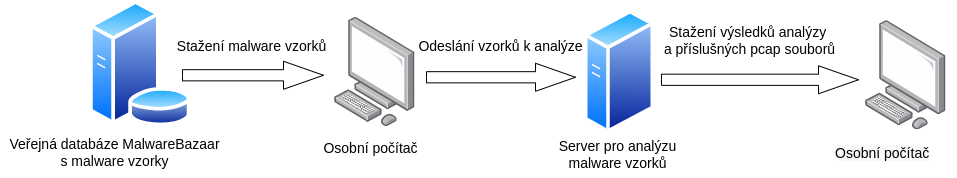
\includegraphics[width=0.8\textwidth]{obrazky/pipeline.png}
	\caption{Proces vytváření datasetů}
    \label{pipeline}
\end{figure}

\section{Stahování malware vzorků}
Prvním krokem je stažení dostatečného počtu malware vzorků pro jednotlivé malware rodiny. Jediným vstupem do toho nástroje od uživatele je tedy pouze textový soubor, který obsahuje
jména rodin. Všechny vzorky jsou stahovány z veřejně dostupné databaze \textit{MalwareBazaar}\footnote{\href{https://bazaar.abuse.ch/}{https://bazaar.abuse.ch/}}. Tato databáze je 
bezplatná a lze stahovat neomezený počet vzorků na rozdíl od jiných databazí jako například \textit{VirusTotal}\footnote{\href{https://www.virustotal.com/gui/home/upload}{https://www.virustotal.com/}}.

Názvy rodin malware musí být stejné jako je specifikuje \textit{MalwareBazaar}, aby nedošlo k nějaké záměně s jiným druhem malwaru. Každý vzorek je poté stažen, jako zaheslovaný zip soubor, aby omylem nedošlo k 
jeho něchtěnému spuštění. Vzorky jsou uloženy podle rodin, aby z důvodu jednoduššího vyhledávání. Jediným omezením je maximalní počet malware vzorků stažených pro jednu rodinu, který činí 1000 vzorků.

\section{Analýza vzorků}
%popsat pcapy, jak probíha analyza, sandboxy
V dalším kroku je nutné veškeré stažené vzorky analyzovat. Každá analýza je prováděna v sandbox prostředení, aby nedošlo k žádnému poškození uživatelského počítače.
Použitým sandbox prostředím pro analýzu je nástroj zvaný \textit{Triage}\footnote{\href{https://tria.ge/dashboard}{https://tria.ge/dashboard}}. Tento nástroj byl vybrán kvůli jeho škálovatelnosti a rychlosti, 
ale především kvůli jeho komplexnímu API rozhraní.

Pro každý vzorek jsou provedeny dvě automatické dynamické analýzy (odkaz na kapitolu) ve dvou různých virtuálních prostředích a jedna statická analýza (ta ovšem není pro tuhle práci tak důležítá, proto se jí dále nebudeme zabývat). 

Celkový proces od nahrání vzorku až po vytoření výsledné zprávy lze vidět na obrázku \ref{Analysis_diagram}. Z něj je patrné, že probíhájí dvě oddělené analýzy. První analýza je prováděno na virtuálním stroji, kde beží 
systém Windows 7 a druhá analýza je prováděna v prostředí se systémem Windows 10.

\begin{figure}[h]
	\centering
        \includegraphics[width=0.6\textwidth]{obrazky/diagram.pdf}
	\caption{Proces analýzy malware vzorků}
    \label{Analysis_diagram}
\end{figure}

Poté, co je vzorek odeslán k analýze, tak je nejprve naplánovaná jeho statická analýza. Po skončení této analýzy je vzorek odeslán k dynamické analýze. Každá analýza se sestáva z extrakce malware vzorku, ze zip archivu. A jeho následného spuštění v čistém prostředí. Poté je zaznamenávána veškerá síťová komunikace a také veškerá aktivita, ke které dojde.
Z obou analýz je pak vygenerována výsledná zpráva.
\section{Výstup programu}
% Popsat pcapy co je v report souborech a k cemu jsou pcapy asi
% konecny vystup programu, rolozeni struktury
%Jak je možné vidět na obrázku \ref{Analysis_diagram}, tak výstupem, který lze ze sandboxu dostat jsou souhrné výsledky analýzy. Tyto výsledky představují soubor (zpráva, anglicky \textit{report}), který popisuje chování malwaru, 
Jak je možné vidět na obrázku \ref{Analysis_diagram}, tak výstupem po skončení dynamické analýzy jsou různé soubory (nebo-li zprávy, anglicky \textit{reports}). Pro účel téhle práce jsou však důležité pouze dva druhy těchto souborů.

Prvním souborem, který je pro tuhle práci relevantní, je soubor obsahující výstup dynamické analýzy. Triage sandbox poskytuje výsledek této analýzy v několika různých formátech jako je třeba XML, JSON či PDF (výstup reportu, který je pak převeden do formátu PDF lze vidět na obrázku ...).
Formát PDF není vhodný z důvodů dalšího zpracování, které bude v následujících fázích potřebné. Nelze z něj jednodušše programově vytáhnout informace. Proto je výsledek analýzy stažen ve formátu JSON.

Mezi významné informace, které lze z toho souboru vyčíst, patří název malware rodiny a krátky popis této rodiny malware. Dále potom ndikátory kompromitace (\texttt{Indicators of Compromise}, zkráceně IoC), 
jsou to tedy hlavně IP adresy a domény, na které se malware snažil připojit a vést jejich prostřednictvím útok. Dále poté může obsahovat navštívené webové stránky a mnoho dalších informací.

\begin{figure}[h]
	\centering
        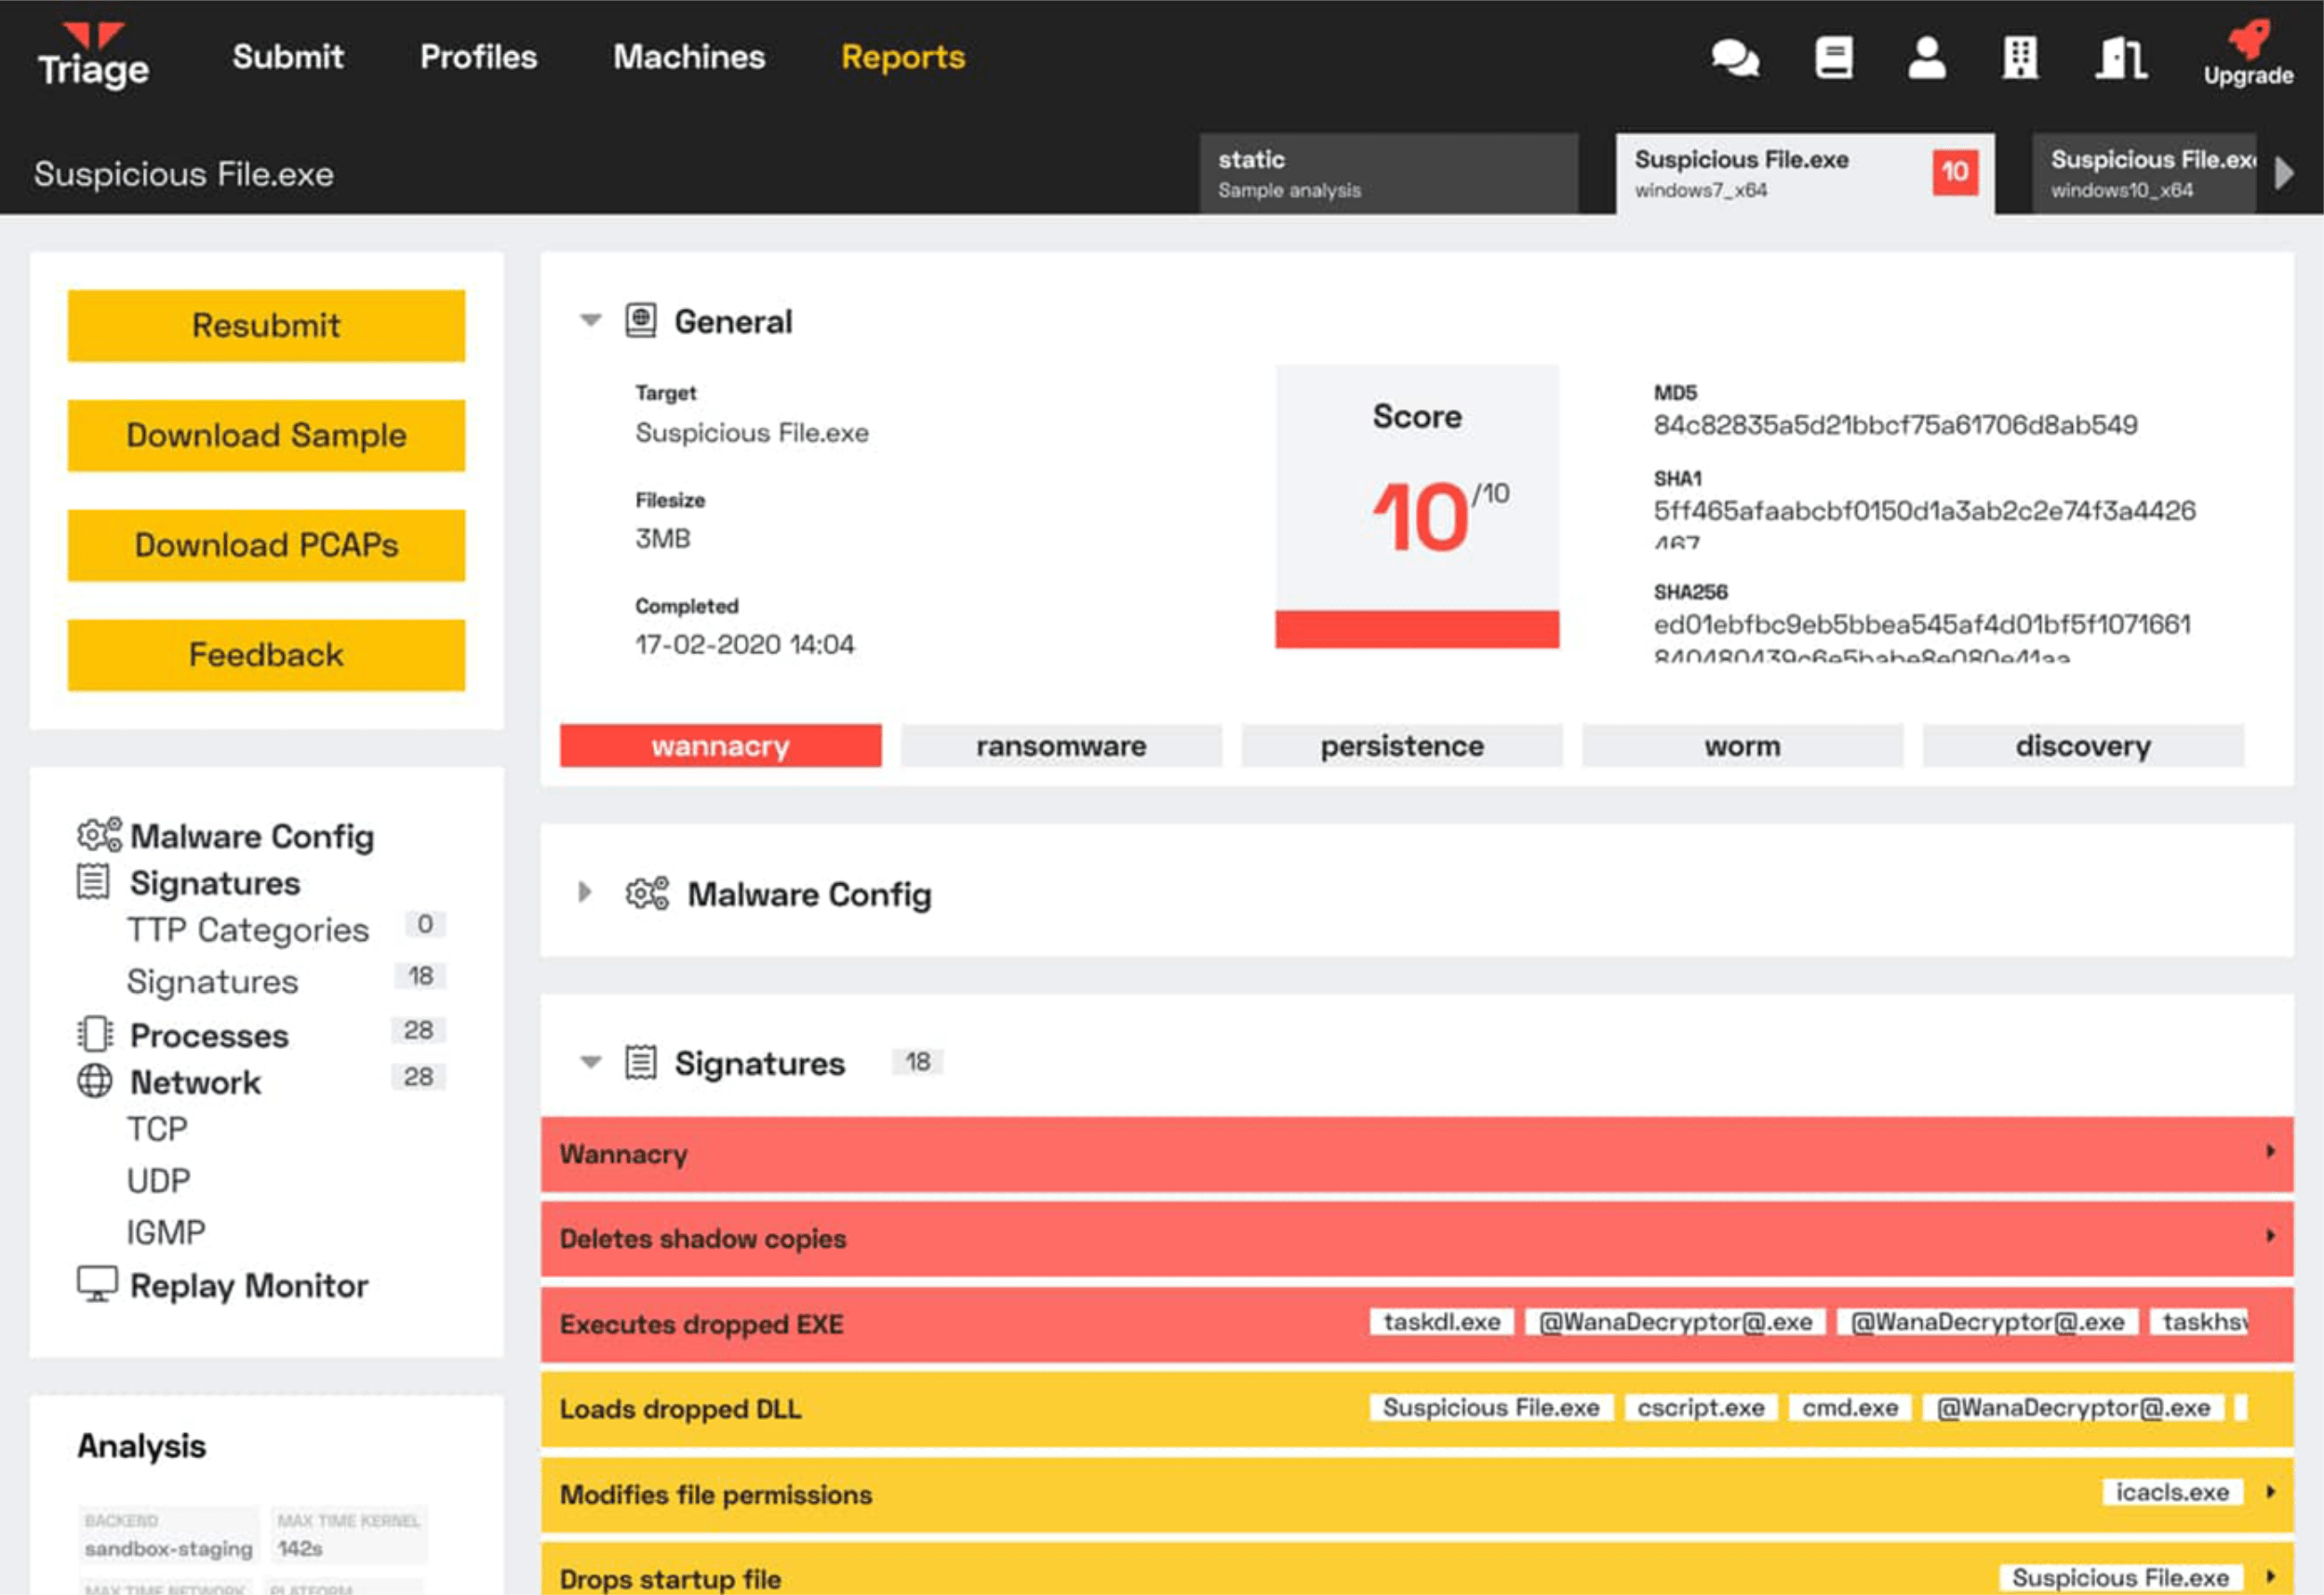
\includegraphics[width=0.7\textwidth]{obrazky/3-triage-report.png}
	\caption{Snímek obrazovky s výsledky z dynamické analýzy}
    \label{Report_image}
\end{figure}

Druhým typem souboru, který je zásadním pro další zpracování jsou soubory typu \texttt{PCAP}. Pro každý malware vzorek jsou staženy dva PCAP soubory.
Tyto soubory obsahují zachycenou síťovou komunikaci ve formě paketů. Tyto soubory lze analyzovat pomocí nástroje \textit{Wireshark}\footnote{\href{https://www.wireshark.org/}{https://www.wireshark.org/}}, 
kde si lze vyfiltrovat komunikaci dle potřeby.

\newpage
\section{Využité technologie}

Veškeré skripty jsou napsány v programovacím jazyce \textbf{Python}. Tento jazyk byl zvolen hned z několika důvodů.
Především ale kvůli jeho jednoduchosti a známosti. Dále taky kvůli knihovnám pro práci s HTTP a posíláním dat po síti.
Velkou výhodou byla také implemetace oficiálního API (aplikačního webového rozhraní z anglického \textit{Application Programming Interface}) klienta pro webové rozhraní 
\texttt{tria.ge}\footnote{\href{https://tria.ge/dashboard}{https://tria.ge/dashboard}}. 
Hlavní využívanou knihovnou je tedy knihovna \textbf{tiage}. Dále se hojně využívá knihovna \textbf{requests} \footnote{\href{https://requests.readthedocs.io/en/latest/}{https://requests.readthedocs.io/en/latest/}}
pro posílaní HTTP požadavků a zpracování jejich odpovědí.

\subsection*{Triage}
Triage je knihovna sloužící ke komunikaci s aplikačním webovým rozhraním Hatching Triage. Tato knihovna usnadňuje práci s analýzou malware vzorků.
Její hlavní použití je tedy odesílaní vzorků k analýze a následné stáhnutí statických výsledků této analýzy a souborů se zachycenou síťovou komunikací v 
podobě paketů, nebo-li souborů s příponou \textit{.pcap}. Hlavní výhodou této knihovny je jednoduchá komunikace s API rozhraním a možnost extrakce všech důležitých
informací z analýzy.

\subsection*{Requests}
Requests je jednoduchá, ale efektivní knihovna pro práci s HTTP/1.1 požadavky a pro spracování odpovědí. Je zde podpora všech typů požadvků, jako jsou
třeba GET, POST, PUT, DELETE a mnoho dalších. Pro potřeby této práce byly použity pouze požadavky typu GET a POST. Dále byly taky využity možnosti
pro spracování odpovědi, ověření zda je spojení stále aktivní a nakonec samotné vytažení a uložení dat.\\ 

Mezi další knihovny, které byly v jisté malé míře použity patří:
\begin{itemize}
    \item Knihovna \textbf{csv}\footnote{\href{https://docs.python.org/3/library/csv.html}{https://docs.python.org/3/library/csv.html}}\\Pro usnadění práce s vytvořenými logovacími soubory.
    \item Knihovna \textbf{pathlib}\footnote{\href{https://docs.python.org/3/library/pathlib.html}{https://docs.python.org/3/library/pathlib.html}}\\Pro vytváření vnořených adresářových struktur a ověřování existence adresářů.
    \item Knihovna \textbf{json}\footnote{\href{https://docs.python.org/3/library/json.html}{https://docs.python.org/3/library/json.html}}\\Slouží pro k převodu slovníků na formát JSON a lepší extrakci informací z tohoto formátu.
\end{itemize}



%Cca 4 stranek
    
\chapter{Závěr}
Max 1 stranka \cite{Pysny}
Popsat co se bude dělat dál jak se bude pokracovat.
TODO



%===============================================================================

% Pro kompilaci po částech (viz projekt.tex) nutno odkomentovat
%\end{document}
